\documentclass[spanish, fleqn]{article}
\usepackage{babel}
\usepackage[utf8]{inputenc}
\usepackage{amsmath,amsfonts}
\usepackage{enumitem}
\usepackage[colorlinks, urlcolor=blue]{hyperref}
\usepackage{fourier}
\usepackage[top = 2.5cm, bottom = 2cm, left = 2cm, right = 2cm]{geometry}
\usepackage{graphicx}
\newcommand{\num}{6}

\title{Estructuras Discretas \\
       Tarea \#\num \\
       $``$\textit{Don Grafo ataca!}$"$}
\author{Andrés Navarro \\ 201673001-K}
\date{}

\begin{document}
\maketitle
\thispagestyle{empty}

\begin{enumerate}

%% Pregunta 1
\item Considere \(K_{2n} \) un grafo completo con \(2n\) vértices \((n\in \mathbb{N} )\). Verificar la veracidad de las siguientes afirmaciones:
\begin{enumerate}
\item \(K_{2n}\) contiene al menos un \textit{ciclo hamiltoniano}.

Es verdadero, debido a que la propiedad de un grafo $K_{2n}$ es que sus $2n$ vértices están conectados todos entre sí, por lo que fácilmente, si elegimos un vértice cualquiera, de este podremos llegar a cualquiera de los demás, y de este a cualquier otro que no hayamos visitado. Finalmente cuando lleguemos al último vértice sin visitar, desde este podremos llegar al primero ya que está conectado a todos los demás vértice.
 
\item \(K_{2n}\) contiene al menos un \textit{circuito de Euler}.

Es falso, dado a que para que exista un circuito de Euler, todos los vértices del grafo deben tener grado par. En este grafo, ya que es de tipo $K_{2n}$, cada vértice esta conectado a los demás, y debido a esto, el grado de los vértices será $2n-1$ (ya que no está conectado consigo mismo).

\item \(K_{2n}\) tiene un índice cromático \( \chi'(K_{2n}) = 2n - 1 \) .


\end{enumerate}

\textbf{Pista:} Para \( c) \) puede serle útil utilizar inducción sobre \(n\).

%% Pregunta 2
\item Dado el grafo:
\begin{center}
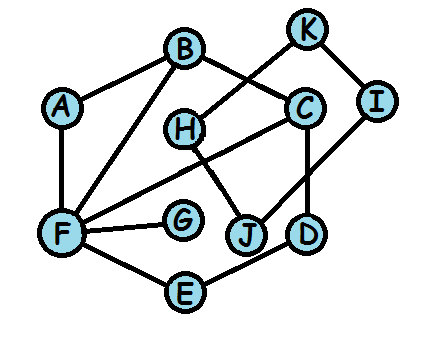
\includegraphics[scale=0.5]{Grafo2}
\end{center}
Determinar: 
\begin{enumerate}
\item{Número cromático.}

$\chi(grafo) = 3$

\item{Índice cromático.}

$\chi'(grafo)= 5$

\item{¿Es un grafo bipartito?}

No lo es, sin embargo, si sólo tomamos en cuenta los vértices $h,k,j,i$, estos si conforman un grafo bipartito.
\item{¿Es este completo?}

No es un grafo completo ya que sus vértices no están conectados a todos los demás.
\end{enumerate}

\end{enumerate}

\end{document}